\section{Monday, October 28, 2019}
Last time, we introduced \vocab{trees}, which are non-linear data structures that can be used to represent relationships between elements. A \vocab{binary tree} is a special type of tree in which each node has at most two children.

\subsection{Tree Traversal}

Unlike like linear data structures, like arrays, we cannot just use a for-loop to iterate over a tree since the data structure is non-linear. Thus, we are motivated to find a new way to traverse the data stored in trees. There are two primary ways in which we can perform tree traversal.

\subsubsection{Breadth-First Search}

\vocab{Breadth-first traversal} starts from a source node, and it visits all nodes that are closest to that source node prior to visiting any nodes that are farther out. In order to illustrate breadth-first traversal, consider the following tree:

\begin{figure}[h]
\centering
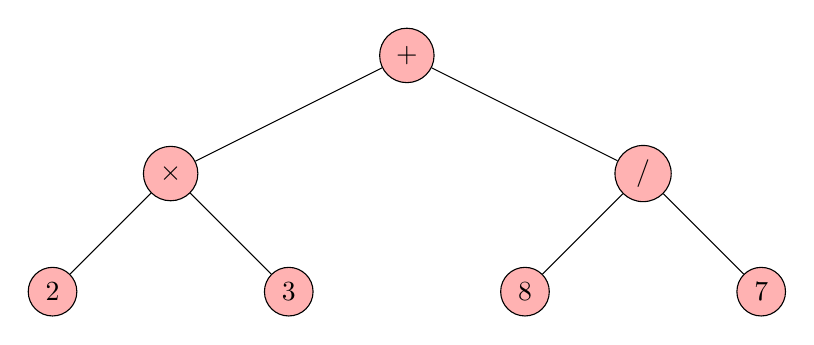
\begin{tikzpicture}[level/.style={sibling distance=60mm/#1}]
\node [circle,draw,fill=red!30] (z){$+$}
  child {node [circle,draw,fill=red!30] (a) {$\times$}
    child {node [circle,draw,fill=red!30] (b) {$2$}
    }
    child {node [circle,draw,fill=red!30] (g) {$3$}}
  }
  child {node [circle,draw,fill=red!30] (j) {$/$}
    child {node [circle,draw,fill=red!30] (k) {$8$}
    }
  child {node [circle,draw,fill=red!30] (l) {$7$}}
};
\end{tikzpicture}
\caption{An Expression Tree}
\end{figure}

Now suppose we begin a breadth-first search traversal starting at the root (the node with the plus sign). In this case, we first visit the root, and we subsequently visit either the node with the multiplication sign or the node with the division sign. The actual order does not matter; the only thing that matters is that the next node visited is the smallest distance away from the root node. Suppose we visit the node with the multiplication sign next. Afterwards, we'll visit the node with the division sign (there is no other node whose distance is only one away from the root, so this is the only candidate). Finally, we'll visit the the nodes whose distances are $2$ away from the root (i.e. the nodes $2, 3, 8, 7$ in any order). 
The key thing to remember when performing a breadth-first search traversal is that the nodes are visited in ascending order of their distance from the root node. 

What are some applications of breadth-first search traversal? One simple example is shown through social networking sites. We can represent all social media profiles with nodes, and we can place an edge between two nodes if the two people represented by those nodes are friends. By performing a breadth-first search, we can figure out how many friends away a given person is from yourself. This can be useful when suggesting friends for you to add. 

\subsubsection{Depth-First Search}

A \vocab{depth-first search traversal} can be further separated into three distinct categories:

\begin{itemize}
    \item In a \vocab{pre-order traversal}, we visit the node that we are currently at first. Subsequently, we recursively visit the left subtree, and we finally recursively visit the right subtree.
    \item In an \vocab{in-order traversal}, we recursively visit the left subtree followed by the node we are currently at, and we finally visit the right subtree.
    \item In a \vocab{post-order traversal}, we recursively visit the left subtree followed by a recursive visit to the right subtree. Finally, we visit the node we are currently at last.
\end{itemize}

\noindent In order to keep track of the three different types of depth-first search traversal, note that the left subtree is \textit{always} visited before the right subtree. Also, the order in which we visit node we are currently at can be determined from the name of the traversal (in a ``pre-order traversal," we visit the node we are currently at first, whereas in a ``post-order traversal", we visit the node we are currently at last).

Once again, consider the same tree from the breadth-first search example:

\begin{figure}[h]
\centering
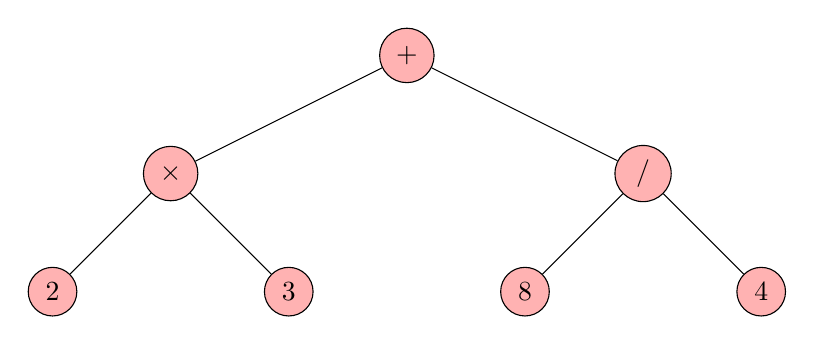
\begin{tikzpicture}[level/.style={sibling distance=60mm/#1}]
\node [circle,draw,fill=red!30] (z){$+$}
  child {node [circle,draw,fill=red!30] (a) {$\times$}
    child {node [circle,draw,fill=red!30] (b) {$2$}
    }
    child {node [circle,draw,fill=red!30] (g) {$3$}}
  }
  child {node [circle,draw,fill=red!30] (j) {$/$}
    child {node [circle,draw,fill=red!30] (k) {$8$}
    }
  child {node [circle,draw,fill=red!30] (l) {$4$}}
};
\end{tikzpicture}
\caption{An Expression Tree}
\end{figure}

Let's trace what happens under the three different types of depth-first search traversal:

\begin{itemize}
    \item In a pre-order traversal, we visit the node we are currently at first, and we subsequently process the left subtree followed by the right subtree. Since we are starting the search at the root, the node with the plus sign is processed first. Subsequently, we make a recursive call on the left subtree. Now to process the node with the multiplication sign, we perform the exact same procedure. We process the node we are currently at first (which is the node with the multiplication sign), and we make a call to the left and right subtrees. This processes the nodes $2$ and $3$ in that order. Finally, there are no more nodes left in the left subtree of the plus symbol, so now we perform a recursive call on the right subtree of the plus node. Similar to the left subtree, we end up processing the division node followed by the $8$ node, and finally the $4$ node. Thus, the final order in which nodes are processed in a pre-order traversal is given by $+, \times, 2, 3, /, 8, 4$. 
    \item In an in-order traversal, we recursively visit the left subtree, then the node we at, and finally the right subtree. In the tree above, we make recursive left calls until we hit the $2$ leaf node. Next, we process the $\times$ node as well as the $3$ node. At this point, we have finished processing the $+$ node's left subtree call. Next, we process the $+$ node, and we finally process $8$ node followed by the $/$ node and $4$ node. Thus, the final order in which the nodes are processed is given by $2, \times, 3, +, 8, /, 4$. 
    \item In a post-order traversal, we process the left subtree, the right subtree, and finally the node we are currently at. In this case, note that the root is always processed last. First, we make a recursive call to the left subtree rooted at $\times$. When processing this subtree, we make another recursive call to the left, and we end up processing $2$ first. Next, we perform the $\times$ node's right subtree call, which results in processing the node $3$. Next, we process the $\times$ node. Finally, we procses the right subtree of $+$ in a similar manner, and we finally process the root node. The final order in which nodes are processed is given by $2, 8, \times, 8, 4, /, +$. 
\end{itemize}

\subsection{Binary Tree Terminology}

Here, we introduce some more terminology that is used to describe binary trees. 

The \vocab{level} of a node is a measure of the node's distance from the root. Observe that there is a natural recursive definition for the level of a node. If the node is the root of the tree, then its level is $1$. Otherwise, the node's level is one plus the level of its parent's level. \\

The \vocab{height} of a tree is the maximum level of any node in the tree.

A tree is called \vocab{degenerate} provided that most of the nodes only have one child. Here is an example of a degenerate tree:

\begin{figure}[h]
\centering
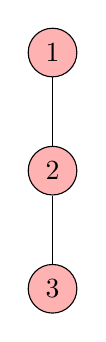
\begin{tikzpicture}[level/.style={sibling distance=60mm/#1}]
\node [circle,draw,fill=red!30] (z){$1$}
  child {node [circle,draw,fill=red!30] (a) {$2$}
    child {node [circle,draw,fill=red!30] (b) {$3$}
    }
};
\end{tikzpicture}
\caption{A Degenerate Tree}
\end{figure}

A degenerate tree is similar to a Linked List in the sense that it is ``approximately linear" (or, like in the case above, it can be linear). Typically, a binary tree being degenerate is an undesirable property to have. The height grows approximately linearly since usually adding a new node increases the height by one. The performance of the tree typically degrades when a tree is degenerate. \\

A tree is called \vocab{balanced} provided that most of its nodes have two children. Here is an example of a tree that is balanced:

\begin{figure}[h]
\centering
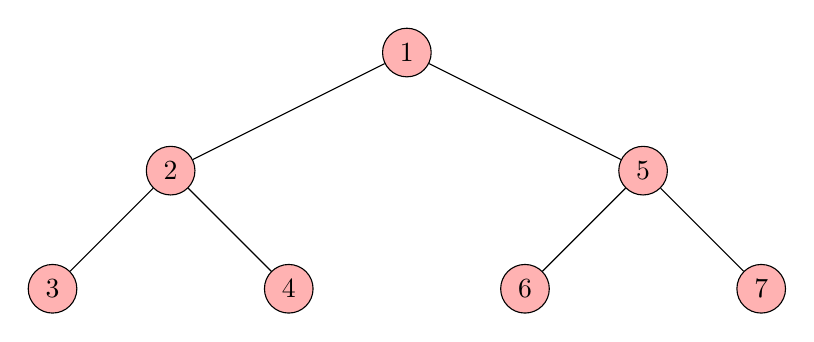
\begin{tikzpicture}[level/.style={sibling distance=60mm/#1}]
\node [circle,draw,fill=red!30] (z){$1$}
  child {node [circle,draw,fill=red!30] (a) {$2$}
    child {node [circle,draw,fill=red!30] (b) {$3$}
    }
    child {node [circle,draw,fill=red!30] (g) {$4$}}
  }
  child {node [circle,draw,fill=red!30] (j) {$5$}
    child {node [circle,draw,fill=red!30] (k) {$6$}
    }
  child {node [circle,draw,fill=red!30] (l) {$7$}}
};
\end{tikzpicture}
\caption{A Balanced Binary Tree}
\end{figure}

Typically, a binary tree being balanced is a desirable property to have. the height grows logarithmically since usually we need to add approximately twice as many nodes as before to increase the height by one. 


A \vocab{full binary tree} is a tree in which every node other than the leaves have two children. The tree above is also a full binary tree, and every full binary tree is balanced. In fact, we can find an explicit formula for the number of nodes in a full binary tree: $n = 2^{h} - 1$, where $h$ is the height of the tree. For example, in the image above, the height of the tree is $3$ (assuming height starts at $1$). Thus, our formula tells us that the tree has $2^{3} - 1 = 7$ nodes, which agrees with our picture above. 

\subsection{Binary Search Trees}

A \vocab{binary search tree} is a data structures that is organized, as its name suggests, in a binary tree. However, they differ in one primary way: the values stored in a binary search tree are always stored in such a way as to satisfy the \vocab{binary-search-tree property}:

\begin{itemize}
    \item For any node $n$, all nodes in the left subtree of $n$ are less than or equal to $n$.
    \item For any node $n$, all nodes in the right subtree of $n$ are greater than or equal to $n$. 
\end{itemize}

Here's an example of a binary search tree:

\begin{figure}[h]
\centering
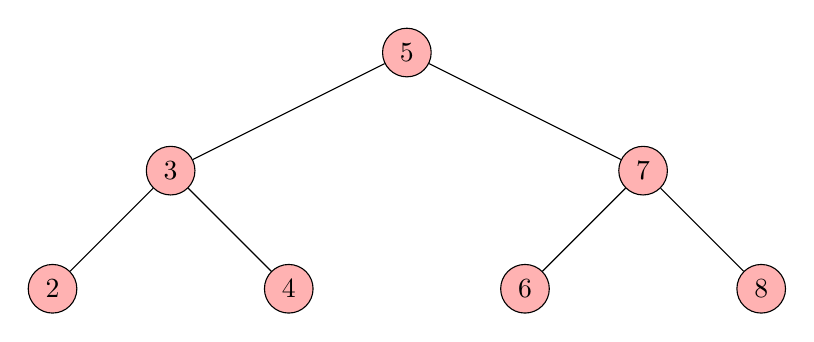
\begin{tikzpicture}[level/.style={sibling distance=60mm/#1}]
\node [circle,draw,fill=red!30] (z){$5$}
  child {node [circle,draw,fill=red!30] (a) {$3$}
    child {node [circle,draw,fill=red!30] (b) {$2$}
    }
    child {node [circle,draw,fill=red!30] (g) {$4$}}
  }
  child {node [circle,draw,fill=red!30] (j) {$7$}
    child {node [circle,draw,fill=red!30] (k) {$6$}
    }
  child {node [circle,draw,fill=red!30] (l) {$8$}}
};
\end{tikzpicture}
\caption{A Binary Search Tree}
\end{figure}

Note that the right subtree the root node contains the values $6, 7,$ and $8$. All three of these values are greater than the root node. On the other hand, all values in the left subtree of the root node are less than the root node. Note that this property does not only apply to the root node but rather every node in the tree. If we choose some arbitrary node in the tree and look at the nodes to the left of it, we should only find smaller values. Likewise, if we choose some arbitrary node in the tree, and we look at nodes to the right of it, we should only find larger values. 

Due to the binary search tree property, performing an in-order traversal on a binary search tree processes the nodes in sorted order. For example, performing an in-order traversal on the tree above processes the nodes in the order $2, 3, 4, 5, 6, 7, 8$. 

How do we search for an element in a binary search tree? We can find an element in a binary search tree by comparing the target value we are searching for with the current node we are at. At each step, this tells us whether our target value should lie in the left subtree or the right subtree (if it exists). For example, suppose we want to look for $4$ in the tree provided above. We start at the root, and we make a comparison with $4$ and $5$. Since $4 < 5$, we know that if $4$ exists, it must lie in the left subtree of $5$. We make a recursive call to the left subtree, and we compare $4$ with $3$. Since $3 < 4$, we recurse on the right subtree of $3$, which happens to be $4$. Note that this is very similar to performing a binary search. We expect the runtime of searching in a binary search tree to be $\O(\log(n))$; however, in the worst case (when the tree is degenerate), the search algorithm runs in $\O(n)$ time. \\

A helpful tool to visualize binary search trees is \url{http://btv.melezinek.cz/binary-search-tree.html}